\documentclass[aspectratio=169,xcolor=pdftex,dvipsnames]{beamer} % dynamic slides
%\documentclass[[aspectratio=169,handout,xcolor=pdftex,dvipsnames,table]{beamer} % handout

%\usepackage{sslides}
\usepackage{multirow}
\usepackage{verbatim}
\usepackage{amssymb,amsmath}

\usepackage{graphicx}
\usepackage{tikz}

%% to support German characters like äöü 
%\usepackage[]{fontenc}
%\usepackage[latin1]{inputenc} 
%\usepackage[austrian]{babel}

%% graphics
\usepackage{graphicx}
\graphicspath{
    {images/}
}

%%----------------------------------------------------------------
%% comment if fancyheadings.sty is not installed (e.g., for MikTex)
%% you can change the logo in the file fancyheadings.tex
%\input{includes/fancyheadings}

\newcommand{\jname}[1]{\textsf{#1}}

%% most beamers can't project decent colors so I set them to max!
%% redefine emph color
%\definecolor{Emph}{rgb}{1,0,0}  %red
\definecolor{Emph}{rgb}{0.7,0.1,0.1}  %softer red for display
\renewcommand{\emph}[1]{\textcolor{Emph}{\bf\textit{#1}}}

%% define color for slide titles
%\definecolor{Title}{rgb}{0,0,1}  %blue
\definecolor{Title}{rgb}{0.2,0.2,0.6}  %softer blue for display
\definecolor{Gold}{RGB}{255,215,0}
%\definecolor{Title}{rgb}{1,0,0}  %red

\newcommand{\jemph}[1]{\textcolor{Blue}{\textbf{#1}}}

\newcommand{\jconstantname}[1]{\textsf{#1}}
\newcommand{\jDefine}[1]{{\bf #1}}
%\input{../preamble/jgreek.tex}
%\input{../preamble/jsymbols.tex}

% SPACING
\newcommand{\spac}[1]{{\makebox[#1]{}}}
\newcommand{\jblankline}{\ \\ \ \\ }
%\renewcommand{\newpage}{\vfill\pagebreak}
\newcommand{\novspace}{\vspace{-.125in}} %use after description environment.
\newcommand{\centerone}[1]{{{\makebox{\ }}{\hfill #1\hfill}{\makebox{\ }}}}
\newcommand{\centertwo}[2]{{{#1}\hfill{#2}\hfill{\makebox{\ }}}}

% FONTS
\newcommand{\bi}[1]{\mbox{\boldmath $#1$}} % bold italic
\newcommand{\rmitem}[1]{\item[{{\rm #1}}]} % use in: description

%---------------------------------------------------------------------------------------------------

%%%%%%%%%%%%%%%%%%%%%%%%%%%%%%%%%%%%%%%%%%%%

\title{\textbf{Mathematics, Physics, Programming\\ and Methodology of Science}}
\author{\textbf{\Large Under construction\\ \ \\Jan Plaza}
\ \\ \ \\ \ \\
github.com/plazajan}
%\date{January 10, 2025
%\\ \ \\ \ \\ \ \\
%\tiny{\copyright 2025 Jan Plaza, licensed under CC BY 4.0}


\begin{document}

\maketitle

%----------------------------------------------------------------------------------------------------
%----------------------------------------------------------------------------------------------------
%%%%%%%%%%%%%%%%%%%%%%%%%%%%%%%%%%%

\begin{frame}
\frametitle{}

\begin{center}
\Huge{Mathematics}
\end{center}



\end{frame}

%----------------------------------------------------------------------------------------------------
\begin{frame}
\frametitle{Ellipse}

\begin{columns}
\column{0.5\linewidth}

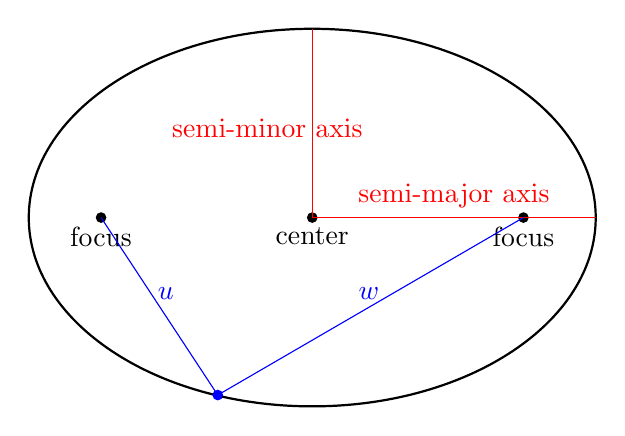
\begin{tikzpicture}[scale=0.6]

%\draw[line width=0.1pt,gray!30,step=1mm] (-6,-4) grid (6,4);
%\draw[help lines] (-6,-4) grid (6,4);

\draw[thick,xscale=1, yscale=0.666] (0,0) circle[radius=6];
\draw[fill] (0, 0) circle[radius=0.1];
\draw[fill] (4.47, 0) circle[radius=0.1];
\draw[fill] (-4.47, 0) circle[radius=0.1];
\node[below] at (0,0) {center};
\node[below] at (4.47,0) {focus};
\node[below] at (-4.47,0) {focus};

\draw[red] (0,0) -- (0,4);
\node[red] at (-0.95,1.9) {semi-minor axis};
\draw[red] (0,0) -- (6,0);
\node[red] at (3,0.45) {semi-major axis};

\draw[fill,blue] (-4.47,0) -- (-2,-3.757) circle[radius=0.1] -- (4.47,0);
\node[blue] at (-3.1,-1.6) {$u$};
\node[blue] at (1.2,-1.6) {$w$};


\end{tikzpicture}

\column{0.5\linewidth}
\begin{itemize}
\item
Draw a circle on a rubber sheet,\\
and stretch it horizontally\\
-- you get an ellipse.
\item
Draw a circle\\
 on a vertically stretched rubber sheet,\\
and let it shrink\\
 -- you get an ellipse.
\item
\textcolor{blue}{$u+w=\text{constant}$}
 \item
 When the foci coincide,\\ the ellipse is a circle.
\end{itemize}

\end{columns} 

\end{frame}

%----------------------------------------------------------------------------------------------------

\begin{frame}
\frametitle{}

Consider an ellipse with the foci at $(-f,0)$ and $(f,0)$\\
on a Cartesian plane, where $f\ge 0$.\\
\ \\
Such an ellipse has a center at $(0,0)$ and is symmetric with respect to:
\begin{itemize}
\item
    point symmetry with respect to $(0,0)$,
\item
    reflection with respect to the $x$-axis,
\item
    reflection with respect to the $y$-axis.
\end{itemize}

\end{frame}

%----------------------------------------------------------------------------------------------------

\begin{frame}
\frametitle{}

Consider an ellipse with the foci at $(-f,0)$ and $(f,0)$
on a Cartesian plane, where $f\ge 0$.\\
\ \\
left vertex, right vertex - the points where the ellipse intersects the $x$-axis.\\
lower vertex, upper vertex - the points where the ellipse intersects the $y$-axis.\\

\begin{itemize}
\item
$a$ - semi-major axis - the distance from the center to the right (or left) vertex.
\item
$b$ - semi-minor axis - the distance from the center to the upper (or lower) vertex.
\item
$c$ - linar eccentricity - the distance from the center to a focus.
\item
$A$ - aphelion - the bigger of the distances from the foci to the right vertex.
\item
$P$ - perihelion - the smaller of the distances from the foci to the right vertex.
\item
$e$ - eccentricity = $c/a$.
\end{itemize}

\end{frame}

%----------------------------------------------------------------------------------------------------

\begin{frame}
\frametitle{}

$2c + 2(a-c) = 2 \sqrt{b^2 + c^2}$ -- from Pythagorean equation.\\
So, $2a = 2 \sqrt{b^2 + c^2}$\\
So, $a = \sqrt{b^2 + c^2}$\\
So, $a^2 = b^2 + c^2$\\
\ \\
$P = a-c$\\
\ \\
$A = a+c$\\
\ \\
$a = (A+P)/2$\\
\ \\
$c = a-P = (A+P)/2 - P = (A-P)/2$\\
\ \\
$b^2 = a^2 - c^2 = ((A+P)/2)^2 - ((A-P)/2)^2 = 4 AP/4 = AP$\\
So, $b = \sqrt{AP}$\\
\ \\
$e = c/a = \sqrt{a^2-b^2} / a = \sqrt{1- (b^2)/(a^2)}$\\
So, $c = ae = \sqrt{a^2-b^2}$

\end{frame}

%----------------------------------------------------------------------------------------------------

\begin{frame}
\frametitle{}

A parametric equation of a circle with radius $r$ and the center at $(0,0)$:\\
$x = r \cos t$,\\
$y = r \sin t$,\\
where $t$ in $[0, 2\pi)$.\\
\ \\
A parametric equation of ellipse with semi-major axis a and semi-minor axis $b$
and the center at $(0,0)$:\\
$x = a \cos t$,\\
$y = b \sin t$,\\
where $t$ in $[0, 2\pi)$.\\
\ \\
Exercise\\
\begin{itemize}
\item
Find a parametric equation of an ellipse with semi-major axis $a$ and semi-minor axis $b$
and the center at $(-C,0)$, where $C$ is a given number.
\item
Find a parametric equation of an ellipse with semi-major axis $a$ and semi-minor axis $b$
and the right focus in the center of the coordinate system.
\end{itemize}

\end{frame}

%----------------------------------------------------------------------------------------------------


\begin{frame}
\frametitle{Vectors and matrices in $R^2$}

Adding vectors: ...\\
\ \\
Length/magnitude of a vector: $|(x,y)| = \sqrt{x^2 + y^2}$\\
\ \\
A unit vector in the direction of vector $(x,y)$:\\
$v = |v|*u$, where $u$ is the unit vector in the direction of $v$\\
\ \\
2x2 matrix \ 
$M = \bigl[\begin{smallmatrix} a&b \\ c&d \end{smallmatrix}\bigr]$\\
Determinant of this matrix: $\det M = ad - bc$\\
\ \\
Area of a parallelogram spanned by two vectors 
= the absolute value of the determinant of the matrix with such column vectors.

\end{frame}

%----------------------------------------------------------------------------------------------------

%%%%%%%%%%%%%%%%%%%%%%%%%%%%%%%%%%%

\begin{frame}
\frametitle{}

\begin{center}
\Huge{Physics}
\end{center}

\end{frame}

%----------------------------------------------------------------------------------------------------

\begin{frame}
\frametitle{Newtonian mechanics, selected laws}

\begin{itemize}
\item
A body not subject to forces is at rest or moves straight at a constant speed.
\item
$F = ma$
\item
Law of gravity: $F = G Mm / (r^2)$
\end{itemize}

Velocity is a vector $(v_x,v_y)$ - may vary with time.\\
$v_x$ - horizontal speed, $v_y$ - vertical speed.\\
Speed is a scalar - the length/magnitude of velocity.\\
\ \\
Acceleration is a vector $(a_x, a_y)$\\
$(a_x, a_y)$- horizontal and vertical acceleration.\\
\ \\
For a body moving on a straight line, $(v_x,v_y)$ and $(a_x,a_y)$ are parallel.\\
For a body moving on a circular orbit, $(v_x,v_y)$ and $(a_x,a_y)$ are perpendicular.\\
For a body moving on a curve, $(v_x,v_y)$ and $(a_x,a_y)$ are not parallel.

\end{frame}

%----------------------------------------------------------------------------------------------------

\begin{frame}
\frametitle{}

Change of position after time $dt$ :\\
$dx = v_x * dt$\\
$dy = v_y * dt$\\
\ \\
Change of velocity after time $dt$ :\\
$dv_x = a_x * dt$\\
$dv_y = a_y * dt$\\
\ \\
Acceleration of a mass $m$ orbiting a stationary mass $M$ while at a distance $r$.\\
$a_x = -G*M*x/r^3$\\
$a_y = -G*M*y/r^3$\\
\ \\
Centripetal force - the force that makes the body to follow a curved path:\\
$F = ma = mv^2/r$

\end{frame}

%----------------------------------------------------------------------------------------------------

\begin{frame}
\frametitle{}

%  x
%----> ^
%     /|
%  r / | y
%   /  | 
%Sun   |

$r = (x,y)$\\
$\hat{r} = (x/r, y/r)$  \ \ -- unit vector in the direction of $r$\\
\ \\
$\vec{F} = M\vec{a}$                          \ \ -- vector equation\\
\ \\
$F = (GMm / r^2)$                    \ \ -- scalar equation\\
$\vec{F} = (GMm / r^2) * (- \hat{r})$      \ \   -- vector equation\\
\ \\
$m\vec{a} = - (GMm / r^2) * \hat{r}$        \ \  -- vector equation\\
$\vec{a}  = - (GM  / r^2) * \hat{r}$       \ \   -- vector equation\\
$a_x = - (GM  / r^2) * x/r = -GMx/r^3$ \ \-- scalar equation\\
$a_y =                       -GMy/r^3$ \ \ -- scalar equation\\
\ \\
In our simulation:\\
$v_x := v_x + a_x t$        \ \            -- scalar equation\\
$v_y := v_y + a_y t$        \ \             -- scalar equation

\end{frame}

%----------------------------------------------------------------------------------------------------

\begin{frame}
\frametitle{Planetary motion (celestial mechanics)}

The two-body problem parameters.\ \\
\ \\
$G$ - the gravitational constant $= 6.67430e\!-\!11\ \ \text{m}^3 \text{kg}^{-1} \text{s}^{-2}$.\\
\ \\
$M$ - the bigger mass (Sun, considered stationary)\\
$m$ - the smaller mass (planet, given some initial velocity, subject to $M$'s gravity.)\\
\ \\
$\mu = G(M+m)$ -- gravitational parameter\\
approximately,  $\mu \approx GM$ when $m <\!\!< M$.\\
\ \\
$r$ - the distance between (the centers of) $M$ and $m$ (varies with time)\\
$v$ - speed of m at its orbit around stationary $M$ (varies with time)\\
\ \\
$T$ - orbital period of $m$ in the movement around $M$.\\
$a$ - semi-major axis of the elliptical orbit of $m$ around $M$.

\end{frame}

%----------------------------------------------------------------------------------------------------
\begin{frame}
\frametitle{Kepler's laws, 1609 - 1619}

\begin{columns}
\column{0.5\linewidth}

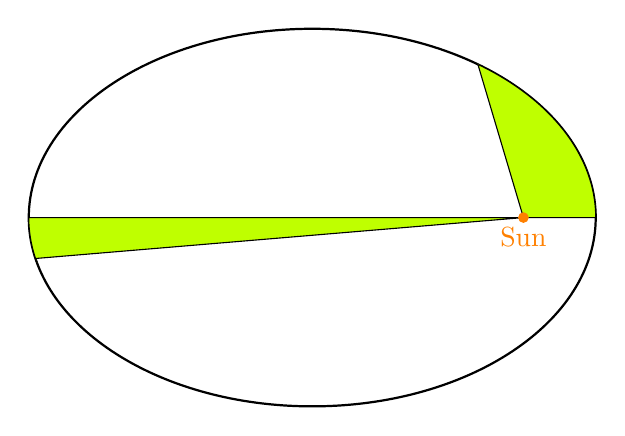
\begin{tikzpicture}[scale=0.6]

%\draw[line width=0.1pt,gray!30,step=1mm] (-6,-4) grid (6,4);
%\draw[help lines] (-6,-4) grid (6,4);

\draw[thick, xscale=1, yscale=0.666] (0,0) circle[radius=6];

\filldraw[fill=lime, xscale=1, yscale=0.666]  (3.5, 4.9) -- (4.47, 0) -- (6, 0) 
                  arc[start angle=0, end angle=54, radius=6];
                  
\filldraw[fill=lime, xscale=1, yscale=0.666]  (-5.85, -1.3) -- (4.47, 0) -- (-6, 0) 
                  arc[start angle=180, end angle=195, radius=6];

\draw[orange,fill] (4.47, 0) circle[radius=0.1];
\node[orange,below] at (4.47,0) {Sun};

\end{tikzpicture}

\column{0.5\linewidth}

Empirical laws of planetary motion\\
(based on Tycho's observations):
\\ \ \\
\begin{enumerate}
\item 
The orbit of a planet is an ellipse\\ with the Sun in a focus.
\item
The line joining a planet and the Sun\\
 sweeps out equal areas\\ during equal intervals of time.\\
(Based on observations of Mars.)
\item 
The square of the orbital period\\ is proportional to\\ the cube of the semi-major axis.
\end{enumerate}

\end{columns} 

\end{frame}

%----------------------------------------------------------------------------------------------------
\begin{frame}
\frametitle{Enhancements to Kepler's laws}

\textbf{Kepler's 2$^{\text{nd}}$ law}, enhanced, vis viva equation:

$$v^2 = G(M+m) \left(\frac{2}{r} - \frac{1}{a}\right)$$

\textbf{Kepler's 3$^{\text{rd}}$ law}, enhanced:

$$ \frac{T^2}{a^3} = \frac{4\pi^2}{G(M+m)}$$

where:\\
$T$ -- orbital period,\\
$a$ -- semi-major axis,\\
$G$ -- gravitational constant,\\
$M,\ m$ -- masses,\\
$v$ -- speed,\\
$r$ -- radius i.e. distance $M$ to $m$.
%$\mu = G(M+m)$ -- gravitational parameter.

\end{frame}


%----------------------------------------------------------------------------------------------------

\begin{frame}
\frametitle{Keplers 1st law:}

   The planet moves on an elliptical orbit with the Sun in one focus.

\end{frame}

%----------------------------------------------------------------------------------------------------

\begin{frame}
\frametitle{Keplers 2nd law}

The planet moves at such a speed that:
\begin{itemize}
\item
    The line connecting the Sun and the planet
    sweeps equal areas in equal periods of time,
\item
    The area of the parallelogram spanned by vectors r and v is constant
\item
    The determinant of the square matrix with columns r and v is constant.
\item
    Vis Viva Equation: $v^2 = G(M+m)(2/r - 1/a)$
\end{itemize}

\end{frame}

%----------------------------------------------------------------------------------------------------

\begin{frame}
\frametitle{Keplers 3rd law}

\begin{itemize}
\item
    $T^2 / a^3 = \text{const}$
\item
    If orbital period in years, and semi-major axis in AU (astronomical units):\\
    $P^2 = a^3$
\item
    $T^2 / a^3 = 4 \pi^2 / (G(M+m)) $\\
    i.e. $T = 2 \pi \sqrt{a^3 / (G(M+m) }$\\
    (If using $G$ in $\text{m}^3 / (\text{kg} * \text{s}^2)$, make sure to use m, s, kg everywhere.)
\end{itemize}

\end{frame}

%----------------------------------------------------------------------------------------------------

\begin{frame}
\frametitle{}

In the case of circular orbits, the orbital period can be easily derived from:\\
$F = mv^2/r$ (centripetal)\\
$F = GMm/(r^2)$ (gravitational)\\
\ \\
We can verify $T^2 = a^3$ for Mars:\\
Mars' sami major axis = 1.524 AU, so its orbital is\\
$T = \sqrt{1.524^3} \approx 1.88$ years.

\end{frame}

%----------------------------------------------------------------------------------------------------

\begin{frame}
\frametitle{The maximum speed of a planet (at the perihelion)}

Vis Viva Equation: $v^2 = G(M+m)(2/r - 1/a)$.\\
\ \\
So, \\
$v_{\text{max}} = \sqrt{G(M+m)(2/P - 1/a) }$ \   where $P =$ perihelion distance.

\end{frame}

%----------------------------------------------------------------------------------------------------

\begin{frame}
\frametitle{Orbit's parameters, from mass, perihelion and maximum speed}

Solve the equation above for $a$:\\
$a = PG(M+m) / (2G(M+m)-P*v_{\text{max}}^2)$\\
\ \\
$c = a - P$ \ \ -- the linear eccentricity, i.e. center-to-focus distance

$A = a + c$ \ \ -- Aphelion distance (biggest distance from the Sun)

$b = \sqrt{A*P}$  \ \ -- semi-minor axis
    
$T = \sqrt{ 4\pi^2a^3 / (G(M+m)) }$ \ \ -- orbital period in seconds

\end{frame}

%----------------------------------------------------------------------------------------------------

\begin{frame}
\frametitle{Mass of the Sun, Earth, Mars, Jupyter}

Can be calculated from the Earth-Sun distance and Earth's orbital period.\\
$T^2 / a^3 = 4 \pi^2 / (GM)$ because $M>\!\!>m$ (mass of Sun $>\!\!>$ mass of Earth)\\
$T$ - Earth's orbital period\\
$a$ - Earth's semi-major axis $\approx$ distance to Sun\\
$T,\  a$ are observable.\\
From the equation, one can calculate the mass of the Sun.\\ 
\ \\
Exercise
\begin{itemize}
\item
Calculate the mass of the Earth
from the distance to the Moon and the Moon's orbital period
\item
Calculate the mass of Mars can be calculated 
from the distance to its moon Phobos and Phobos' orbital period.
\item
Calculate the mass of Jupyter can be calculated 
from the distance to its moon Io and Io's orbital period.
\end{itemize}
\end{frame}

%----------------------------------------------------------------------------------------------------

%%%%%%%%%%%%%%%%%%%%%%%%%%%%%%%%%%%

\begin{frame}
\frametitle{}

\begin{center}
\Huge{Computational Experiment}
\end{center}

\end{frame}

%----------------------------------------------------------------------------------------------------
\begin{frame}
\frametitle{Kepler's world - a computer simulation to test Kepler's laws}



\begin{columns}
\column{0.45\linewidth}
      \includegraphics[width=70mm]{keplersWorld.png}
\column{0.55\linewidth}
   

\begin{itemize}
\item
A computer simulation of orbits resulting from the continuing local effect of the Newton's law of gravity $F = G\frac{M m}{r^2}$
\item
Tests if the simulated planets obey (global) Kepler's laws 1 and 3.
\item 
The screenshot on the left:\\ \textcolor{darkgray}{Mercury}, \textcolor{YellowOrange}{Venus}, 
\textcolor{blue}{Earth}, \textcolor{red}{Mars}.
\item
Verified ellipses with the Sun in one focus.
\item
Orbital periods in days,\\ simulation vs. actual:\\
\textcolor{darkgray}{Mercury: 88.77 vs. .87.97 (0.91\% error)}\\
\textcolor{YellowOrange}{Venus: 225.46 vs. 224.7 (0.34\% error)}\\
\textcolor{blue}{Earth: 365.97 vs 365.26 (0.2\% error)}\\
\textcolor{red}{Mars: 687.85 vs 686.98 (0.13\% error)}
\item
Available at \texttt{github.com/plazajan}
\end{itemize}
\end{columns} 

\end{frame}

%----------------------------------------------------------------------------------------------------


{
\setbeamertemplate{background}
{
    \includegraphics[width=\paperwidth]{Screenshot2.jpg}
}
\begin{frame}
\frametitle{\textcolor{white}{Kepler's World -- a computer simulation to test Kepler's laws}}
 
\end{frame}
}

%---

\begin{frame}
\frametitle{}

For every planet, Kepler's World
\begin{itemize}
\item 
draws the Sun as a white dot,
\item
draws in pink the ellipse predicted by Kepler's 1st law and its two foci.
\item
draws in pink a straight line segment, whose length is proportional to the orbital period of the planet predicted by Kepler's 3rd law; the greater the area sweep speed predicted by Vis Viva equation (from Kepler's 2nd law), the higher the line.
\item 
Uses Newton's law of gravity to simulate the movement of the planet and
marks it position (for Mars -- in red),
\item
also graphs the value of the area sweep speed, from time 0 to the time of completion of the orbit.
\end{itemize}

\end{frame}

%The program draws in pink the elliptical orbit with the foci
%as predicted by Kepler's laws,
%then it simulates the planet movement based on Newton's laws
%and draws the scaled down path of the planet,
%after which it calculates and draws the foci.
%If the two graphs coincide, this confirms Kepler's 1st law:
%every planet's orbit is an ellipse with the Sun in one focus.
%
%The 2nd law says that the line from the Sun to the planet
%sweeps equal areas in equal amounts of time.
%This is equivalent to having a constant area-sweep speed.
%The 3rd law says that the square of the orbital period is proportional to
%the cube of the semi-major axis of the elliptical orbit
%(and the constant of proportionality is known).
%The program tests these laws as well.
%It draws in pink a graph showing the prediction from Kepler's laws 
%of how the sweep speed depends on time,
%for times from 0 to the predicted orbital period
%-- this graph is a segment of a straight horizontal line.
%Then, during the simulation, it graphs the sweep speed
%from the beginning to the end of a complete orbital period.
%If the two graphs coincide, this confirms Kepler's 2nd and 3rd laws.
%
%The program also prints information concerning the error of the simulation;
%notice that the scaled down graphs concerning Kepler's 2nd and 3rd laws
%coincide perfectly only because of limited resolution of computer screens,
%while in reality there exists an error.

%----------------------------------------------------------------------------------------------------

%%%%%%%%%%%%%%%%%%%%%%%%%%%%%%%%%%%

\begin{frame}
\frametitle{}

\begin{center}
\Huge{Methodology of Science}
\end{center}

\end{frame}

%----------------------------------------------------------------------------------------------------

\begin{frame}
\frametitle{Natural science}

Natural science describes the natural world:
\begin{itemize}
\item
physics (force, movement, particle, atom, radiation, ...),\\
encompass astronomy and astrophysics,
\item
chemistry (element, molecule, reaction, ...)
\item
biology (cell, organism, species, evolution, ...)
\item
planetary science, \\
encompass Earth, oceanic and atmospheric science.
\end{itemize}

Contrasted with social science:
\begin{itemize}
\item
psychology (behavior of a person),
\item
anthropology, sociology (behavior of a society, culture, ...),
\item
political science (government, policy, ...),
\item
economics (supply, demand, trade, ...)
\end{itemize}

Note: Neuroscience (nervous system, brain, ...) bridges biology and psychology.

\end{frame}



%----------------------------------------------------------------------------------------------------

\begin{frame}
\frametitle{Logic, mathematics, natural science}

Logic guides reasoning in mathematics and in natural science.
\\ \ \\
Mathematics consists of \jemph{theorems}. (For instance, the Pythagorean Theorem.)\\
A theorem is a statement that has a proof based on specific axioms/assumptions.\\
Theorems are universally valid -- true forever and in any place in the universe.\\
Mathematics is a tool used in natural science.
\\ \ \\
Natural science consists of \jemph{laws of science}.\\
%(For instance, the Newton's law of gravity, $F = G\frac{M\cdot m}{r^2}$).
For instance, the Galilean law of addition of velocities: $v = v_1 + v_2$ \\ -- 
a person who walks at 2 mph on a train traveling at 20 mph is moving at 22 mph.\\
A\! law of science is our best description at the\! moment of an\! aspect of the\! natural world.\\
To be a law of science, a statement must be precise, \jemph{falsifiable} and consistent with available data.
The Galilean law of addition of velocities has been falsified and is now considered only an approximate description of reality, applicable to velocities much smaller than the speed of light. Currently, Einstein's theory of relativity provides a new law of addition of velocities. This law may be falsified in the future.
\end{frame}

%----------------------------------------------------------------------------------------------------

\begin{frame}
\frametitle{The scientific method}

Science is built using the \jemph{scientific method}:\\

\begin{itemize}
\item
observe/experiment (obtain empirical evidence/data)
\item
construct a theoretical model, 
\item
make predictions based on the model, 
\item
test the predictions.
\end{itemize}
\end{frame}



%----------------------------------------------------------------------------------------------------

\begin{frame}
\frametitle{Methods of science: }

\begin{itemize}
\item
experimental/observational, 
\item
theoretical/mathematical, 
\item
computational.
\end{itemize}

\end{frame}

%----------------------------------------------------------------------------------------------------

\begin{frame}
\frametitle{Units of measurement and dimensional analysis:}

\jemph{International System of Units (SI)}, base units:\\
Mass: kilogram (kg)  $\approx$ 2 pounds\\
Length: meter (m) $\approx$ 1 yard\\
Time: second (s),\\
(also ampere, kelvin, mole, candela.)
\\ \ \\
Speed -- distance per time:  $\text{m}/\text{s}=\text{m}\cdot \text{s}^{-1}$.\\
Acceleration -- speed change per second: 
$(\text{m}/\text{s})/\text{s} = \text{m}/\text{s}^2=\text{m}\cdot \text{s}^{-2}$.\\
Force -- \  $F = ma$: \ $\text{Newton} = \text{kg}\cdot \text{m}/\text{s}^2 =  \text{kg}\cdot \text{m}\cdot\text{s}^{-2}$.
\\ \ \\
Gravitational constant: $G$,\\
$F = G \frac{Mm}{r^2}$, \\
$\text{kg}\cdot \text{m}\cdot\text{s}^{-2} = \ x\cdot\text{kg}^2\text{m}^{-2}$.\\
So, $G$ has dimension $x = \text{kg}^{-1}\text{m}^3\text{s}^{-2}$.

\end{frame}
%----------------------------------------------------------------------------------------------------

\begin{frame}
Vis Viva Equation -- speed vs. distance from the Sun:\\ 
$v^2 = G(M+m)(2/r - 1/a)$, where $a$ is the length of the semi-major axis,
$(\text{m}\cdot\text{s}^{-1})^2 = \text{kg}^{-1}\text{m}^3\text{s}^{-2}(\text{kg}+\text{kg})(\text{m}^{-1} - \text{m}^{-1})$, i.e.\\
$\text{m}^2\cdot\text{s}^{-4} = \text{kg}^{-1}\text{m}^3\text{s}^{-2}\text{kg}\cdot\text{m}^{-1}$.\\
This does not prove the Vis Viva Equation,\\
but shows there is nothing wrong with its unit dimensions.
\\ \ \\
Orbital period $T = 2 \pi \sqrt{a^3 / (G(M+m))}$\\
$\text{s}=\sqrt{\text{m}^3 (\text{kg}^{-1}\text{m}^3\text{s}^{-2})^{-1}(\text{kg}+\text{kg})^{-1}}$, i.e.\\
$\text{s}=\sqrt{\text{m}^3 \text{kg}\cdot\text{m}^{-3}\text{s}^{2}\text{kg}^{-1}}$.\\
Nothing is wrong with unit dimensions.

\end{frame}

%----------------------------------------------------------------------------------------------------

\begin{frame}
\frametitle{Approximations}

$\pi = \texttt{3.1415926535897932384626433...}$\\
$\pi \approx \texttt{3.14159265}$\\
$\pi \approx \texttt{3.1415927}$\\
$\pi \approx \texttt{3.141593}$\\
$\pi \approx \texttt{3.14159}$\\
$\pi \approx \texttt{3.1416}$\\
$\pi \approx \texttt{3.142}$\\
$\pi \approx \texttt{3.14}$\\
$\pi \approx \texttt{3.1}$\\
$\pi \approx \texttt{3}$\\

\end{frame}

%----------------------------------------------------------------------------------------------------

\begin{frame}
\frametitle{Absolute and relative errors}

Tm -- tera-meter = $10^{12}$ m = 1 000 000 000 000 meters.
\\ \ \\
Neptune's perihelion: \\
4.47 Tm, all digits significant, i.e.\\
$4.47\pm 0.005$ Tm
\\ \ \\
4 470 000 000 000 m \ could be an approximation of either of:
\begin{itemize}
\item
4 465 000 000 000 m\\
absolute error = 4 470 000 000 000 - 4 465 000 000 000 = 5 000 000 000 m\\
relative error = 5 000 000 000 / 4 465 000 000 000 $\approx 0.11\%$.
\item
4 474 999 999 999.99 m\\
absolute error = 4 474 999 999 999.99 - 4 470 000 000 000 = 4 999 999 999.99 m\\
relative error = 4 999 999 999.99 / 4 474 999 999 999 $\approx 0.11\%$.
\end{itemize}

\end{frame}

\begin{frame}
\frametitle{}

Calculations involving approximate values and the estimation of error are subjects of \jemph{numerical analysis}
(which is not in the scope of this presentation).

\end{frame}


%----------------------------------------------------------------------------------------------------

\begin{frame}
\frametitle{Metric prefixes}

\begin{tabular}{ | l | c | l | r | }
\hline
peta & P & $10^{15}$ & 1 000 000 000 000 000 \hspace{3.5cm} \\ \hline
tera & T & $10^{12}$ & 1 000 000 000 000 \hspace{3.5cm} \\ \hline
giga & G & $10^{9}$ & 1 000 000 000 \hspace{3.5cm} \\ \hline
mega & M & $10^{6}$ & 1 000 000 \hspace{3.5cm} \\ \hline
kilo & k & $10^{3}$ & 1 000  \hspace{3.5cm} \\ \hline
hecto & h & $10^{2}$ & 100 \hspace{3.5cm} \\ \hline
deca & da & $10^{1}$ & 10 \hspace{3.5cm} \\ \hline
-- & -- & $10^0$ & 1 \hspace{3.5cm} \\ \hline
deci & d & $10^{-1}$ &  0.1 \hspace{3.2cm} \\ \hline
centi & c & $10^{-2}$ & 0.01 \hspace{3cm} \\ \hline
mili & m & $10^{-3}$ & 0.001 \hspace{2.8cm} \\ \hline
micro & $\mu$ & $10^{-6}$ & 0.000 001 \hspace{2.1cm} \\ \hline
nano & n & $10^{-9}$ & 0.000 000 001 \hspace{1.4cm} \\ \hline
pico & p & $10^{-12}$ & 0.000 000 000 001 \hspace{0.7cm} \\ \hline
femto & f & $10^{-15}$ & 0.000 000 000 000 001 \hspace{0cm} \\ \hline
\end{tabular}

\end{frame}

%----------------------------------------------------------------------------------------------------

\begin{frame}
\frametitle{Floating-point numbers}

Floats are not like reals. Floats implement the IEEE 754-2008 standard.

\begin{itemize}
\item
There are only finitely many floats (of any given type). 
\item
Floats are discrete, while reals are dense and continuous.
\item
The farther from zero -- the more sparse.
\item
There is a biggest numerical float. 
There is a smallest positive float.
\item
Most reals can be only approximated by floats.
\item
There are special float values:\\
 negative zero (-0), infinity (inf), negative infinity (-inf), not-a-number (NaN).
 \item
Often, the actual result of an arithmetical operation on floats\\
 can be only approximated by a float.
\item 
Associativity fails:
(1 + 1e100) + -1e100 = 0 \  while \  1 + (1e100 + -1e100) = 1.
\end{itemize}
For instance, numeric values of ``tiny floats" look as follows on the number line.
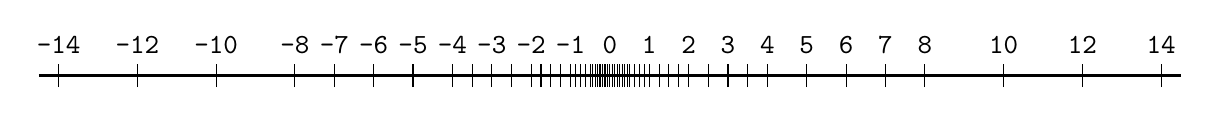
\begin{tikzpicture}[scale=0.5]

\draw[thick] (-14.5,0)--(14.5,0);

\draw (0,-.3)--(0,.3) node[anchor=south] {\texttt{0}};

\draw (0.0625 ,-.3)--(0.0625 ,.3);
\draw (0.125,-.3)--(0.125,.3);
\draw (0.1875 ,-.3)--(0.1875,.3);

\draw (0.25 ,-.3)--(0.25 ,.3);
\draw (0.3125 ,-.3)--(0.3125 ,.3);
\draw (0.375 ,-.3)--(0.375 ,.3);
\draw (0.4375 ,-.3)--(0.4375 ,.3);

\draw (0.5 ,-.3)--(0.5 ,.3);
\draw (0.625 ,-.3)--(0.625 ,.3);
\draw (0.75 ,-.3)--(0.75 ,.3);
\draw (0.875 ,-.3)--(0.875 ,.3);

\draw (1 ,-.3)--(1 ,.3) node[anchor=south] {\texttt{1}};
\draw (1.25 ,-.3)--(1.25 ,.3);
\draw (1.5 ,-.3)--(1.5 ,.3);
\draw (1.75 ,-.3)--(1.75 ,.3);

\draw (2 ,-.3)--(2 ,.3) node[anchor=south] {\texttt{2}};
\draw (2.5 ,-.3)--(2.5 ,.3);
\draw (3 ,-.3)--(3 ,.3) node[anchor=south] {\texttt{3}};
\draw (3.5 ,-.3)--(3.5 ,.3);

\draw (4 ,-.3)--(4 ,.3) node[anchor=south] {\texttt{4}};
\draw (5 ,-.3)--(5 ,.3) node[anchor=south] {\texttt{5}};
\draw (6 ,-.3)--(6 ,.3) node[anchor=south] {\texttt{6}};
\draw (7 ,-.3)--(7 ,.3) node[anchor=south] {\texttt{7}};

\draw (8 ,-.3)--(8 ,.3) node[anchor=south] {\texttt{8}};
\draw (10 ,-.3)--(10 ,.3) node[anchor=south] {\texttt{10}};
\draw (12 ,-.3)--(12 ,.3) node[anchor=south] {\texttt{12}};
\draw (14 ,-.3)--(14 ,.3) node[anchor=south] {\texttt{14}};

\draw (-0.0625 ,-.3)--(-0.0625 ,.3);
\draw (-0.125,-.3)--(-0.125,.3);
\draw (-0.1875 ,-.3)--(-0.1875,.3);

\draw (-0.25 ,-.3)--(-0.25 ,.3);
\draw (-0.3125 ,-.3)--(-0.3125 ,.3);
\draw (-0.375 ,-.3)--(-0.375 ,.3);
\draw (-0.4375 ,-.3)--(-0.4375 ,.3);

\draw (-0.5 ,-.3)--(-0.5 ,.3);
\draw (-0.625 ,-.3)--(-0.625 ,.3);
\draw (-0.75 ,-.3)--(-0.75 ,.3);
\draw (-0.875 ,-.3)--(-0.875 ,.3);

\draw (-1 ,-.3)--(-1 ,.3) node[anchor=south] {\texttt{-1}};
\draw (-1.25 ,-.3)--(-1.25 ,.3);
\draw (-1.5 ,-.3)--(-1.5 ,.3);
\draw (-1.75 ,-.3)--(-1.75 ,.3);

\draw (-2 ,-.3)--(-2 ,.3) node[anchor=south] {\texttt{-2}};
\draw (-2.5 ,-.3)--(-2.5 ,.3);
\draw (-3 ,-.3)--(-3 ,.3) node[anchor=south] {\texttt{-3}};
\draw (-3.5 ,-.3)--(-3.5 ,.3);

\draw (-4 ,-.3)--(-4 ,.3) node[anchor=south] {\texttt{-4}};
\draw (-5 ,-.3)--(-5 ,.3) node[anchor=south] {\texttt{-5}};
\draw (-6 ,-.3)--(-6 ,.3) node[anchor=south] {\texttt{-6}};
\draw (-7 ,-.3)--(-7 ,.3) node[anchor=south] {\texttt{-7}};

\draw (-8 ,-.3)--(-8 ,.3) node[anchor=south] {\texttt{-8}};
\draw (-10 ,-.3)--(-10 ,.3) node[anchor=south] {\texttt{-10}};
\draw (-12 ,-.3)--(-12 ,.3) node[anchor=south] {\texttt{-12}};
\draw (-14 ,-.3)--(-14 ,.3)node[anchor=south] {\texttt{-14}};

\end{tikzpicture}

\end{frame}

%---

\begin{frame}

\begin{center}
\begin{tabular}{ | c || l | l | l | l | l |}
\hline
Sign, Exponent & \ 00 & \ 01 & \ 10 & \ 11 & Explanation\\ \hline 
\hline
0 \ 000 & \ \textbf{0} &\ \ \ 0.0625 &\ \ \ 0.125 &\ \ \ 0.1875 & keep adding 1/16 \\ \hline
0 \ 001 & \ 0.25 &\ \ \ 0.3125 &\ \ \ 0.375 &\ \ \ 0.4375 & keep adding 1/16 \\ 
0 \ 010 & \ 0.5 &\ \ \ 0.625 &\ \ \ 0.75 &\ \ \ 0.875 & keep adding 1/8 \\ 
0 \ 011 & \ \textbf{1} &\ \ \ 1.25 &\ \ \ 1.5 &\ \ \ 1.75 & keep adding 1/4 \\ 
0 \ 100 & \ 2 &\ \ \ 2.5 &\ \ \ 3 &\ \ \ 3.5 & keep adding 1/2 \\ 
0 \  101 & \ 4 &\ \ \ 5 &\ \ \ 6 &\ \ \ 7 & keep adding 1 \\ 
0 \ 110 & \ 8 & \ 10 & \ 12 & \ 14 & keep adding 2 \\ \hline
0 \ 111 & \ inf &\ \ \  NaN &\ \ \  NaN &\ \ \ NaN & special values \\ \hline

1 \ 000 & \textbf{-0} &\ \ -0.0625 &\ \ -0.125 &\ \ -0.1875 & \\ \hline
1 \ 001 & -0.25 &\ \ -0.3125 &\ \ -0.375 &\ \ -0.4375 & \\ 
1 \ 010 & -0.5 &\ \ -0.625 &\ \ -0.75 &\ \ -0.875 & \\ 
1 \ 011 & \textbf{-1} &\ \ -1.25 &\ \ -1.5 &\ \ -1.75 & \\ 
1 \ 100 & -2 &\ \ -2.5 &\ \ -3 &\ \ -3.5 & \\ 
1 \ 101 & -4 &\ \ -5 &\ \ -6 &\ \ -7 & \\ 
1 \ 110 & -8 & -10 & -12 & -14 & \\ \hline
1 \ 111 & -inf &\ \ \  NaN &\ \ \  NaN &\ \ \  NaN &  \\ \hline
\end{tabular}
\end{center}

\end{frame}

%---

\begin{frame}
\frametitle{}

In the previous table, 00, 01, 10, 11 in the header are values of ``fraction", \\ aka ``significand", aka ``mantissa".
\ \\
\begin{center}
\begin{tabular}{| l || l | l | l | l | l | l | l | }
\hline
& \!Sign\! & \!Exponent\! & \!Fraction\! & Total & \!How many\! & \!Min\! pos\! & \!Max \\ \hline
\hline
\!``Tiny floats" & \!1 \!bit\! & \ 3 bits  & \ 2 bits & \ 6\! bits\! & $55 \approx 2^6$ & $2^{-4}$ & \!$14\approx 2^{4}$ \\ \hline
\!1.4.3-minifloats\! & \!1 \!bit\! & \ 4 bits  & \ 3 bits & \ 8\! bits\! & $239 \approx 2^{8}$ & $2^{-9}$ & \!$240 \approx 2^8$  \\ 
\hline
\!Half-precision& \!1 \!bit\! & \ 5 bits  & \!10 bits & \!16\! bits\! & $63487\!\approx\! 2^{16}$\! & $2^{-24}$ & \!$ 65504\! \approx\! 2^{16}$\!  \\ \hline
\!Single-precision\! & \!1 \!bit\! & \ 8 bits  & \!23 bits & \!32\! bits\! & $\approx 2^{32}$ & $2^{-149}$ & \!$ \approx 2^{128}$  \\ \hline
\!Double-prec.& \!1\! bit\! & \!11 bits  & \!52 bits & \!64\! bits\! & $\approx 2^{64}$ & $2^{-1074}$ & \!$\approx 2^{1024}$ \\ \hline
\end{tabular}
\end{center}
\ \\ \ \\
\jemph{Problem.} \ For double-precision floats, calculate:
\begin{enumerate}
\item
the exact number of numeric values other than -0,\\
and the exact maximum numerical value;
\item
the maximum relative error while approximating by a float\\ a real number
 between 1 and the maximum numerical float.
\end{enumerate}

\end{frame}

%----------------------------------------------------------------------------------------------------

\begin{frame}
\frametitle{Discrete vs continuous}

\jemph{Discrete} simulation of a \jemph{continuous} process.

\end{frame}


%----------------------------------------------------------------------------------------------------

\begin{frame}
\frametitle{Recurrent/periodic process}

Recurrent/periodic process - for instance planet's movement around the Sun.

\end{frame}

%----------------------------------------------------------------------------------------------------

\begin{frame}
\frametitle{Qualitative vs. quantitative statements}

\begin{enumerate}
\item 
``a planet moves fastest when close to the Sun" vs. Kepler's 2nd law.
\item
The line joining a planet and the Sun
 sweeps out equal areas during equal intervals of time.
\item 
$v^2 = G(M+m) \left(\frac{2}{r} - \frac{1}{a}\right)$
\end{enumerate}


\end{frame}

%----------------------------------------------------------------------------------------------------

\begin{frame}
\frametitle{Local vs global}

\jemph{Local} effects (of the law of gravity) vs.
\jemph{global} properties (of orbits described by Kepler's laws).

\end{frame}

%----------------------------------------------------------------------------------------------------

\begin{frame}
\frametitle{Visualization vs. simulation.}

\begin{itemize}
\item
Could we make a simulation of planetary motion without a visualization?
\item
Could we make a visualization of planetary motion without an underlying simulation?
\end{itemize}

\end{frame}

%----------------------------------------------------------------------------------------------------

%\begin{frame}
%\frametitle{}
%
%Emergence (of Kepler's laws from Newton's laws) or
%
%reduction of (Kepler's laws to Newton's laws).
%  
%Note: Newton gave a (mathematical) proof, using calculus.
%
%Note: This example is oversimplified. A proper example would be
%the emergence of the theory of gasses from Newtonian mechanics.
%
%\end{frame}

%----------------------------------------------------------------------------------------------------

\begin{frame}
\frametitle{Abstraction and simplification}

\jemph{Abstraction} - the process of removing from consideration those details which have no impact on the answer to the question.

\jemph{Simplification} - the process of removing from consideration those details which have minor impact on the answer to he question, or those which make the problem mathematically or computationally unmanageable.
Simplification amounts to adding the problem new assumptions, which make it simpler.
\\ \ \\
While modeling the planetary motion in the Solar System:
\begin{itemize}
\item
We abstract away the chemical composition of the planet, existence of life, the name of the planet, etc.
\item
We simplify the problem considering only one planet moving around the Sun (a two-body problem).
The two-body problem is mathematically solvable, while a general three body system is chaotic, with an unpredictable behavior in the long term.
\end{itemize}


\end{frame}

\begin{frame}
\frametitle{The Shell Theorem}

\emph{Theorem} (Isaac Newton, 1687)\\
A spherically symmetric body affects external objects gravitationally as though all of its mass were concentrated at a point at its center.
\\ \ \\
We simplify the planetary motion problem assuming that the Sun and the planet are spherically symmetric (as they approximately are.)
\\ \ \\
Then, by the Shell Theorem we perform an abstraction -- we consider point masses instead of three-dimensional bodies.

\end{frame}

%----------------------------------------------------------------------------------------------------

\begin{frame}
\frametitle{Representation}

We assume that the Sun is in the center of a planar Cartesian coordinate system.\\
\ \\
A planet is represented as a point and a velocity vector in 2 dimensions.

\end{frame}


%----------------------------------------------------------------------------------------------------

%\begin{frame}
%\frametitle{Measurements: relative vs. absolute.}

%absolute size/diameter of the Moon.
%Measured in units of length, such as meters.

%????? relative size of the Moon to the size of the Sun -- about equal.\\
%Either one is about 1/2 degree.

%\end{frame}

%----------------------------------------------------------------------------------------------------

\begin{frame}
\frametitle{Ockham's razor}

Given two models that give the same predictions, choose the simpler one.\\
\ \\
For instance, even if the Ptolemaic model of the Sun and planets gave the same predictions 
as the Copernican/x model, we would choose the Copernican/Keplerian model because it is simpler.

\end{frame}

%----------------------------------------------------------------------------------------------------

%\begin{frame}
%\frametitle{}

%\end{frame}

%----------------------------------------------------------------------------------------------------

%\begin{frame}
%\frametitle{}

%\end{frame}

%----------------------------------------------------------------------------------------------------

%\begin{frame}
%\frametitle{}

%\end{frame}



%%%%%%%%%%%%%%%%%%%%%%%%%%%%%%%%%%%%%%%%%%%%

\end{document}

%%%%%%%%%%%%%%%%%%%%%%%%%%%%%%%%%%%%%%%%%%%%
%%%%%%%%%%%%%%%%%%%%%%%%%%%%%%%%%%%%%%%%%%%%
